\documentclass[reprint,superscriptaddress,aps,amsmath,amssymb]{revtex4-1}

\usepackage{graphicx}% Include figure files
\usepackage{placeins}
\usepackage{dcolumn}% Align table columns on decimal point
\usepackage{bm}% bold math
\usepackage{color}
\makeatletter
\setlength{\@fptop}{0pt}
\makeatother
\usepackage{natbib}
%\usepackage[numbers,sort&compress]{natbib}

\usepackage{graphicx}
\usepackage{hyperref}
\usepackage{amsmath}

%\bibliographystyle{spbasic}

\usepackage{titlesec} %\titlespacing{command}{left spacing}{before spacing}{after spacing}[right]
\titlespacing\section{0pt}{10pt}{4pt}
\titlespacing\subsection{0pt}{10pt}{2pt}
\titlespacing\subsubsection{0pt}{10pt}{1pt}

\begin{document}
\title{plant-growing facility Design and Operation}
\author{Jim C. Visschers} \email{jvisschers@uni-mainz.de}
\affiliation{Institut f\"ur Physik, Johannes Gutenberg Universit\"at-Mainz, 55128 Mainz, Germany}
\affiliation{Helmholtz-Institut Mainz, GSI Helmholtzzentrum f\"{u}r Schwerionenforschung GmbH, Mainz 55128, Germany}

\begin{abstract}
Your abstract.
\end{abstract}
\maketitle
\tableofcontents
\section{Introduction}
In this work we present the design, realization and characterization measurements of a plant growing facility. The motivation behind building the plant-growing facility are planned measurements of time-resolved chiral volatile organic compound (VOC) emission measurements from plants within the lab. The growth facility is required to provide an optimal, observable, controllable and importantly, repeatable growing environment for the plants of interest in various growth stages. 

The growth facility needs to fulfill certain requirements in order to be used effectively for the previously mentioned experiments and to be able to facilitate many experimental variations. For instance, individual plants should be in their individual chambers to minimize unintentional cross talk between plants and cross contamination between plants, however the ability to study plant communication through the emissions of VOC's or soil should be an option. A high degree of automation, such as automated watering and an automated day-night cycle, is crucial to ensure optimal and repeatable growth conditions within a lab environment and minimize the need for outside intervention during long-running experiments or multi-week growth stages of certain plant species. 

To accurately, and sufficiently monitor the growing conditions within each individual growing compartment within the plant-growth facility we need to observe some basic environmental parameters. These include: (1) Air temperature, (2) Air humidity, (3) Air Pressure, (4) Light levels, and, (5) Soil humidity levels. These basic measurements are needed to ensure optimal growth conditions within a compartment of the growth-chamber. By also measuring some gasses present within the growth chamber we hope to gain insight into plant VOC emissions corresponding to the environment. The desired gas concentration measurements include: (1) total volatile organic compounds (tVOC), (2) carbon dioxide, (3) nitrogen dioxide, (4) ethyl alcohols, (5) ozone, and finally (6) oxygen. Importantly, from the plant emissions we also hope to gain insight on additional plant conditions that are imposed onto the plants under observation.

In the following sections we will describe the physical design and layout of the plant-growing facility followed by a description of the data handling and measurement scheme as well as a description of the home-made climate sensors. Finally some characterization measurements are presented which are important for the eventual use of plant-growth facility.

\section{Plant growing facility}
\begin{figure}
    \centering
    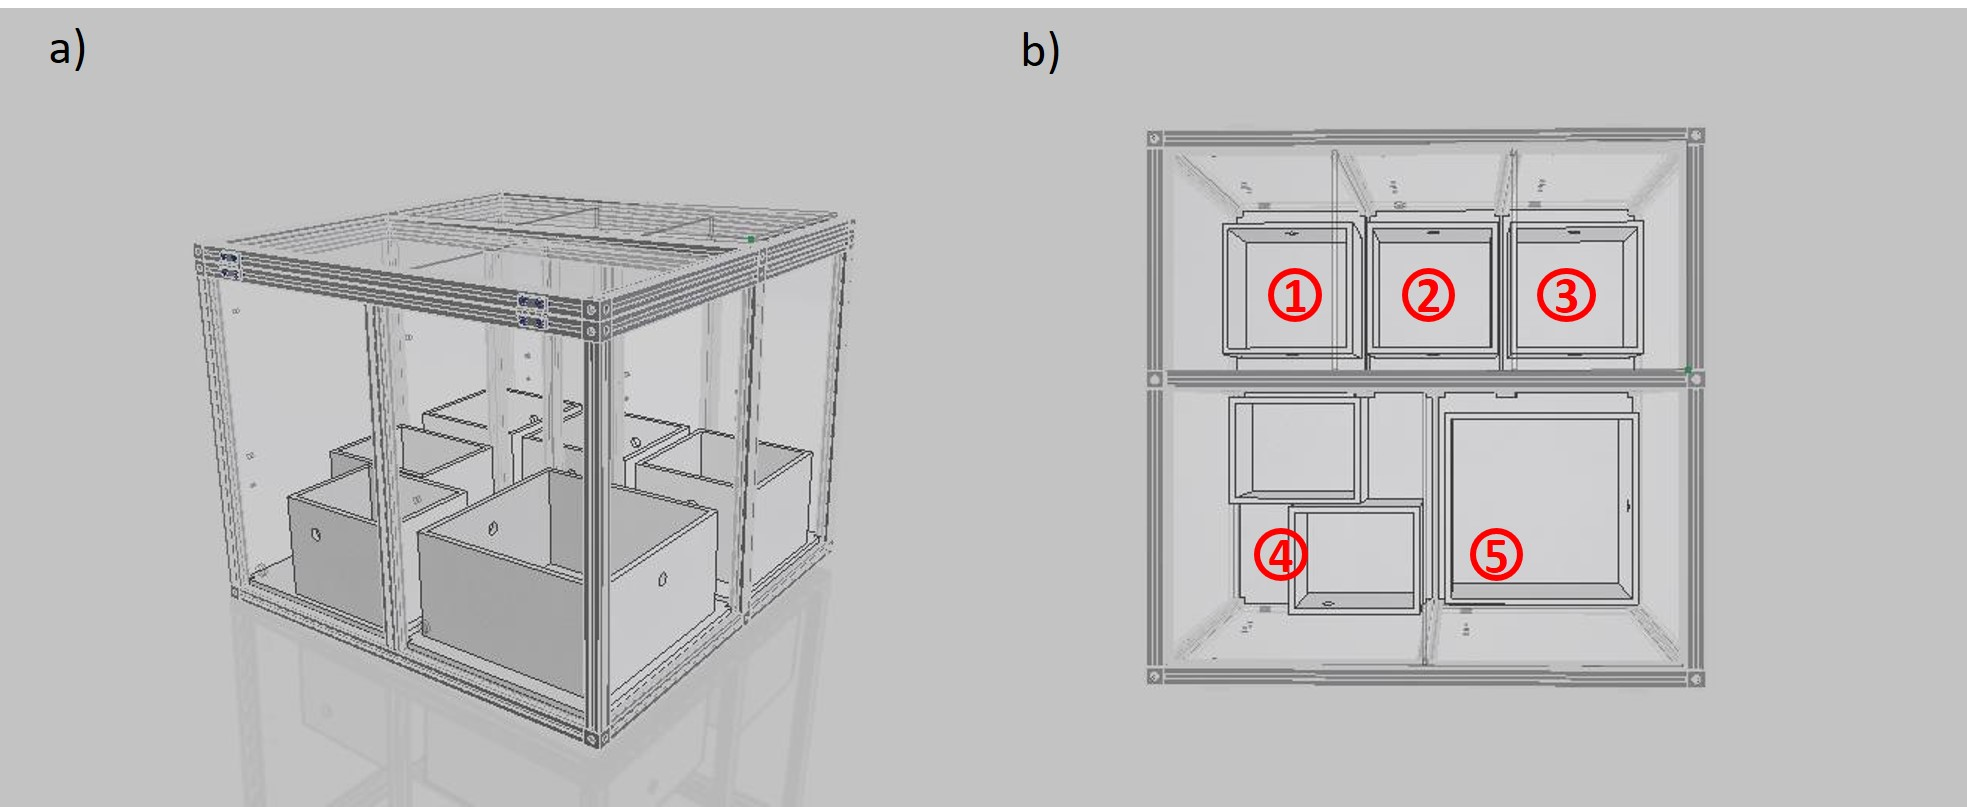
\includegraphics[width=1\linewidth]{growbox.jpg}
    \caption{Design schematics of the plant-growing facility. \textbf{a)} Perspective view of the plant-growing facility. \textbf{b)} Top view of the plant-growing facility. The different growth compartments are labeled 1 through 5. Compartments 1,2, and 3 are individual compartments allowing to house a single plants each. Compartment 4 is able to accommodate two plants with separated soil containers. Compartment 5 features a single, large soil container that can house two plants at the same time.}
    \label{fig: Growth Box}
\end{figure}
\begin{figure*}
    \centering
    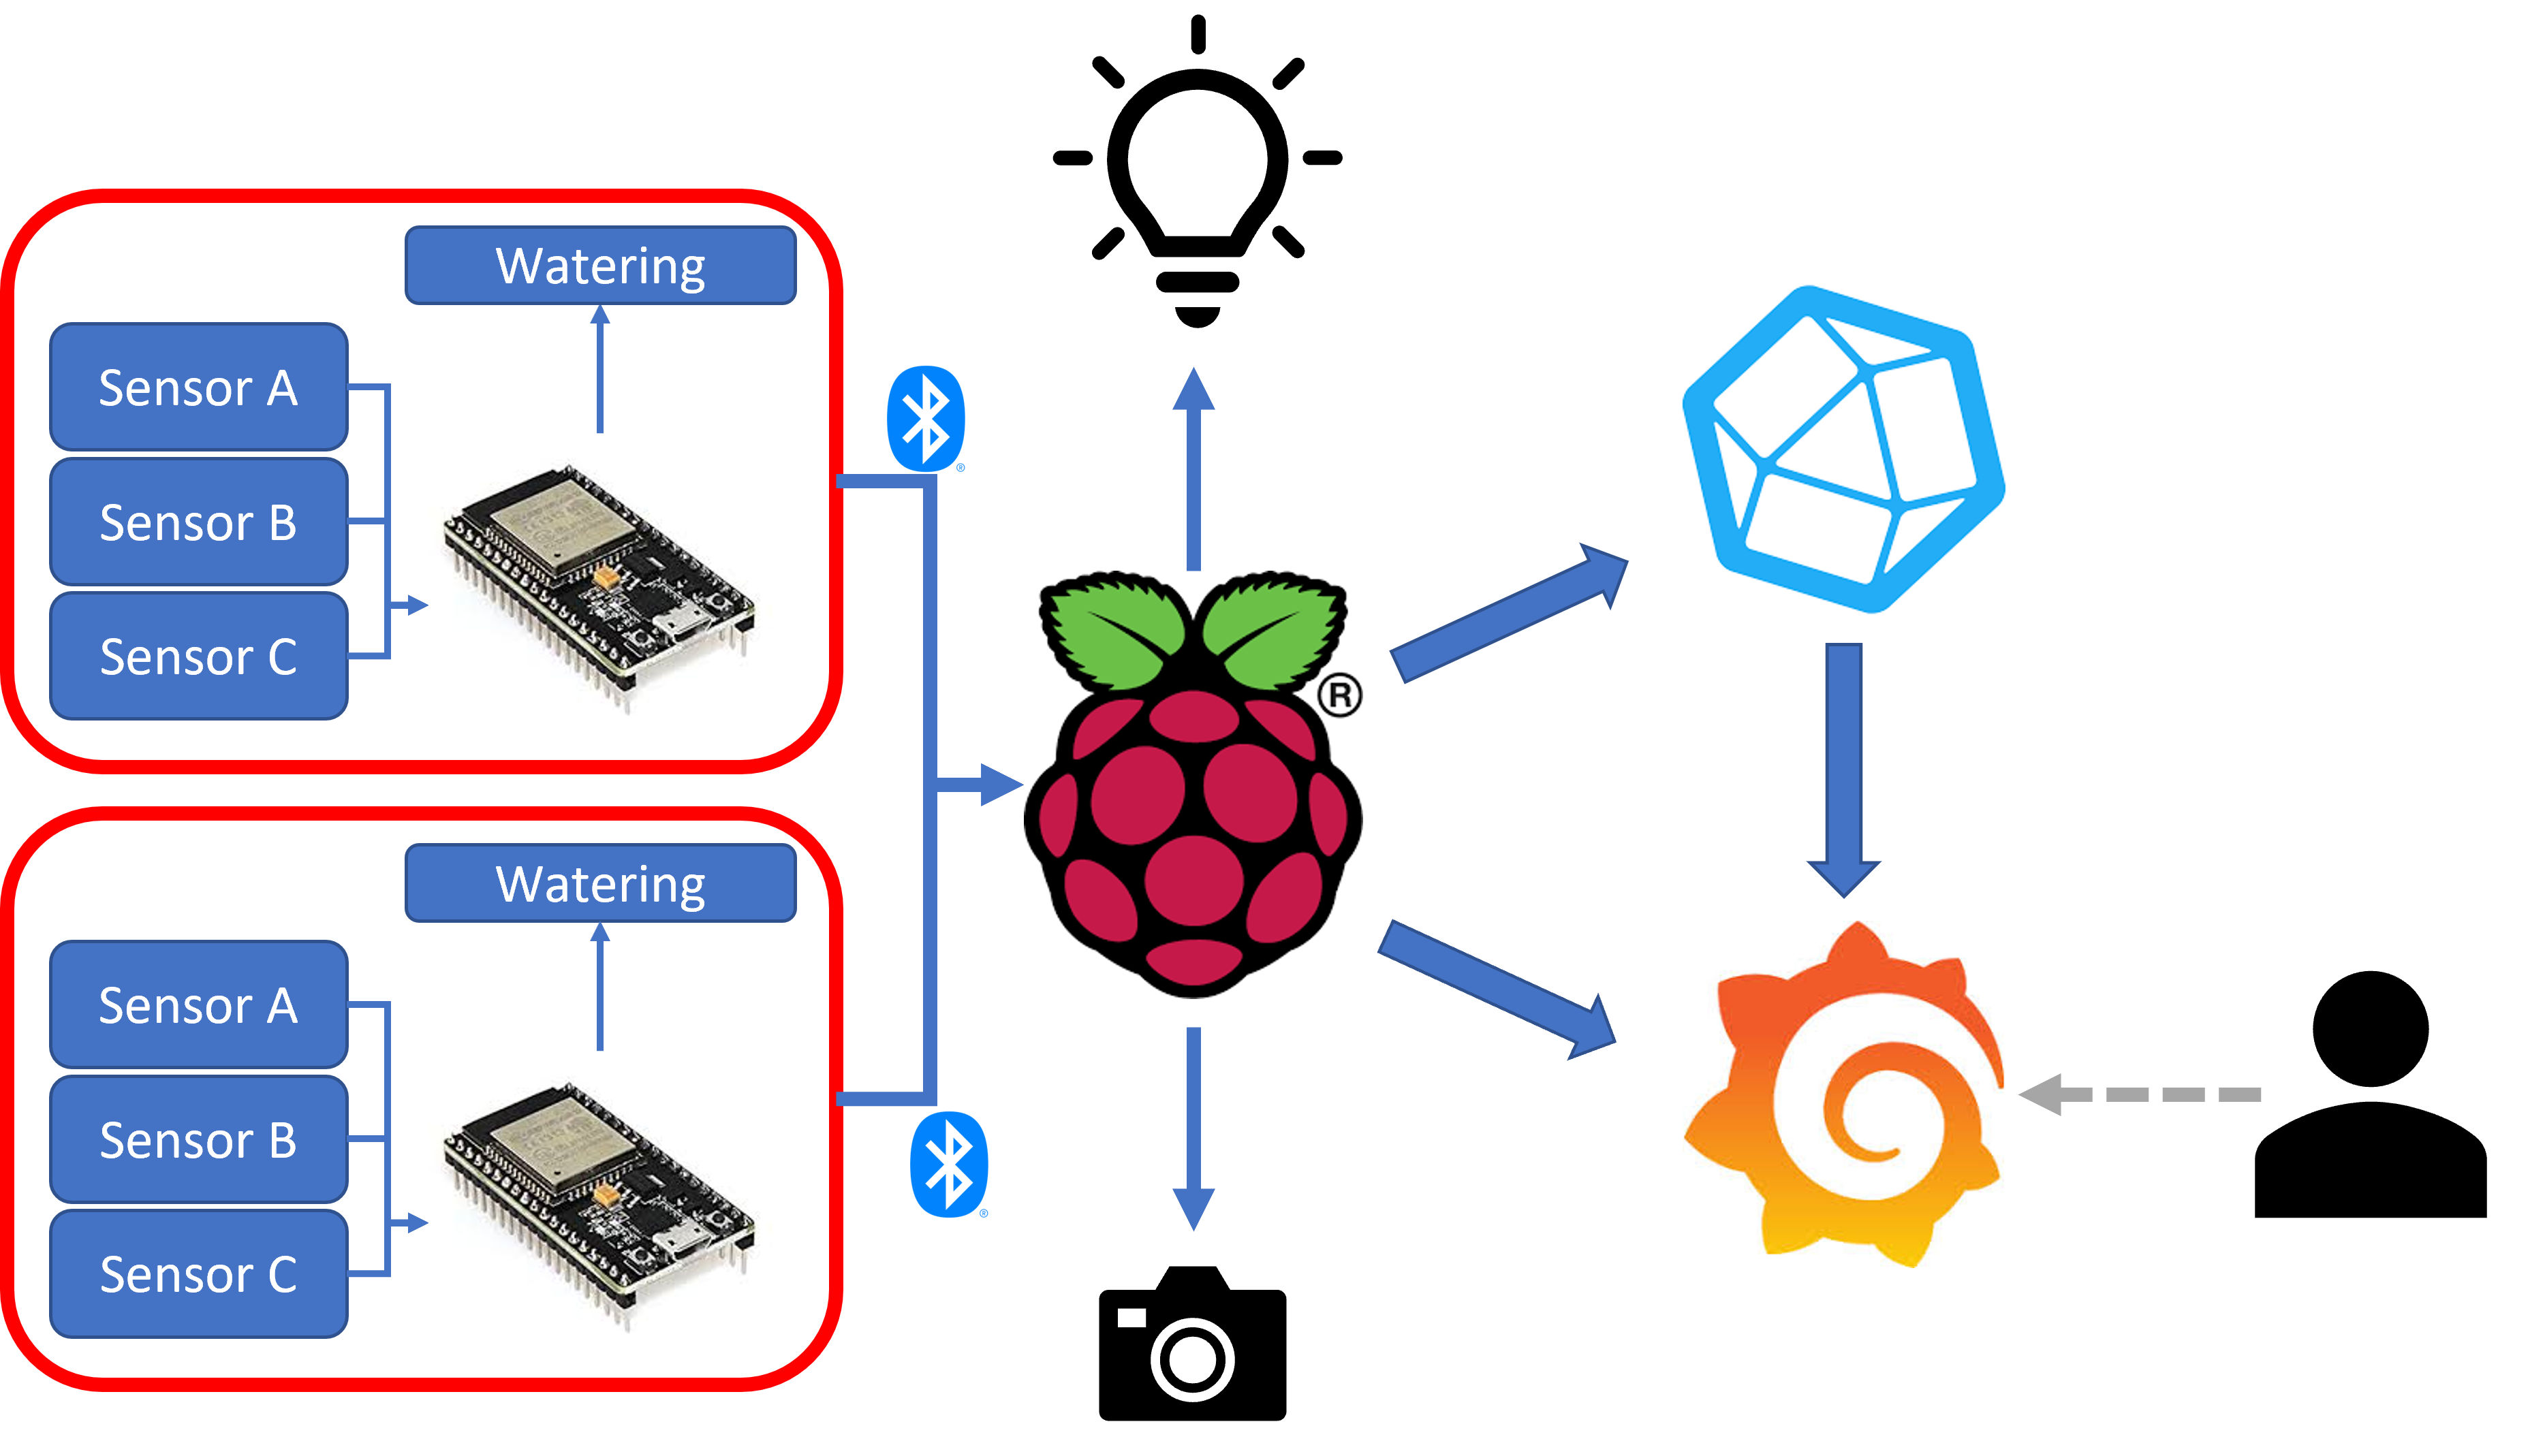
\includegraphics[width = \linewidth]{Data overview.png}
    \caption{Visualisation of the experimental control and data flow for the plant-growing facility. The red boxes represent individual compartments of the growth-box facility. Each functional growth chamber has an ESP-32 based sensor board which measures the climate parameters within each box and controls the watering of the soil. Each sensor board advertises the various sensor values in a Bluetooth Low Energy (BLE) service. The BLE service is read-out periodically by a Raspberry-Pi\,4 which saves the data into an InfluxDB database. The Raspberry-Pi\,4 also controls the light cycle of the plant growing facility and has the capabilities of controlling a camera to periodically image the growing plants. Finally the Raspberry-Pi\,4 hosts a Grafana server that visualizes the data from the ESP-32 sensor boards and is remotely accessible to anyone within the institutes network.}
    \label{fig:Data overview}
\end{figure*}
We designed a plant-growing facility consisting of five separated growth chambers, a side- and top-view of the design shown in Fig. \ref{fig: Growth Box}. Three of the five compartments house individual plants and allow for controlled studies of individual plants. The fourth chamber houses two plants but with individual soil containers and allows for communication between two plants through VOC emissions. The fifth and final chamber in the plant-growing facility is also able to house two plants sharing the air and soil allowing for both soil and VOC communication between plants. The footprint of the complete plant-growing facility is 75\,cm\,x\,75\,cm with a height of 60\,cm. The soil containers have a height of 17cm. The footprint of the soil containers in the individual growth compartments (1, 2, and 3) have a size of 20\,cm\,x\,20\,cm. The soil containers in the fourth compartment have a footprint of  20\,cm\,x\,16\,cm, and finally, the soil box in the combined compartment has a footprint of 30\,cm\,x\,30\,cm.

The frame of the plant-growing facility is made from Thorlabs optical rails while the windows and soil containers are made in-house and are made from perspex and PVC respectively.
We are able to access the growth compartments in the box through two top folding doors. The first of which gives access to the three individual compartments and the second one opens up the two double compartments. Electrical access is provided through a 2\,cm hole in one of the outside window panels of each individual growth chamber at the heights of the top of the soil compartments. Two smaller holes provide access for a sampling tube for sampling of the plant emissions at the top and base of the plant respectively. A final hole at the height of the top of the soil container provides access for a watering tube.

Light is provided from high-efficiency, plant growth optimized LED lighting (NEONICA Growy). The lights consume 13\,W/m. The ceiling of each growth compartment is lined with 20 cm strips of LED lighting totalling 1\,m. In growth chamber 3 (Fig\,\ref{fig: Growth Box}b) we put an additional 0.6\,m of LED lighting controlled separately form the regular lighting which gives us the ability to induce light stress in the plant growing in that compartment. To maximize the amount of light within the growth chamber we coat the insides of each compartment with aluminium foil. This subsequently limits the light leakage form the plant-growing facility \footnote{Much to the delight of the other occupants in the lab.}.

\section{Measurements, Data logging and handling}
Structured experimental controls and a clear data collection scheme are crucial for the ease-of-use of the growth box. In an effort to retain oversight we take a top down approach: we use a Raspberry-Pi\,4 to collect, store and visualize all the relevant data from the different growth compartments. Furthermore, it is in control of all -facility wide- processes (such as the light cycle). Each individual growth compartment is fitted with a home-made climate sensor that observes the relevant environmental parameters within said growth compartment and reports them to the Raspberry-Pi\,4, the climate sensors also regulate processes specific to a single growth-box (e.g. watering of the plants). A visualisation of the controls and data flow is given in Fig.\,\ref{fig:Data overview}.

\subsection{Raspberry-Pi\,4}
A Raspberry-Pi\,4 platform is used as the main data center for the plant-growing facility. It is ideal for this specific project because it is a lightweight and affordable computer platform that supports Bluetooth Low Energy (BLE) and accommodates remote access via SSH. The Raspberry-Pi\,4 is used to collect and store the sensor data from the individual growth chambers in a database. It controls the light cycle of the plant-growth facility through a USB connected relay circuit. The four relays allow for four independent light cycles within the plant growing facility. Currently the growth facility is set-up on a single light cycle and a separate relay is used to control additional lights in compartment 3 (Fig.\,\ref{fig: Growth Box}) which enables us to induce light stress in that specific compartment.
We make extensive use of the Linux job scheduler Cron to perform periodic tasks, such as turning on and off the lights in the plant growing facility, monitoring the climate parameters and pushing/pulling new versions of the GitHub repository.

\subsection{Climate sensor}
\begin{figure}
    \centering
    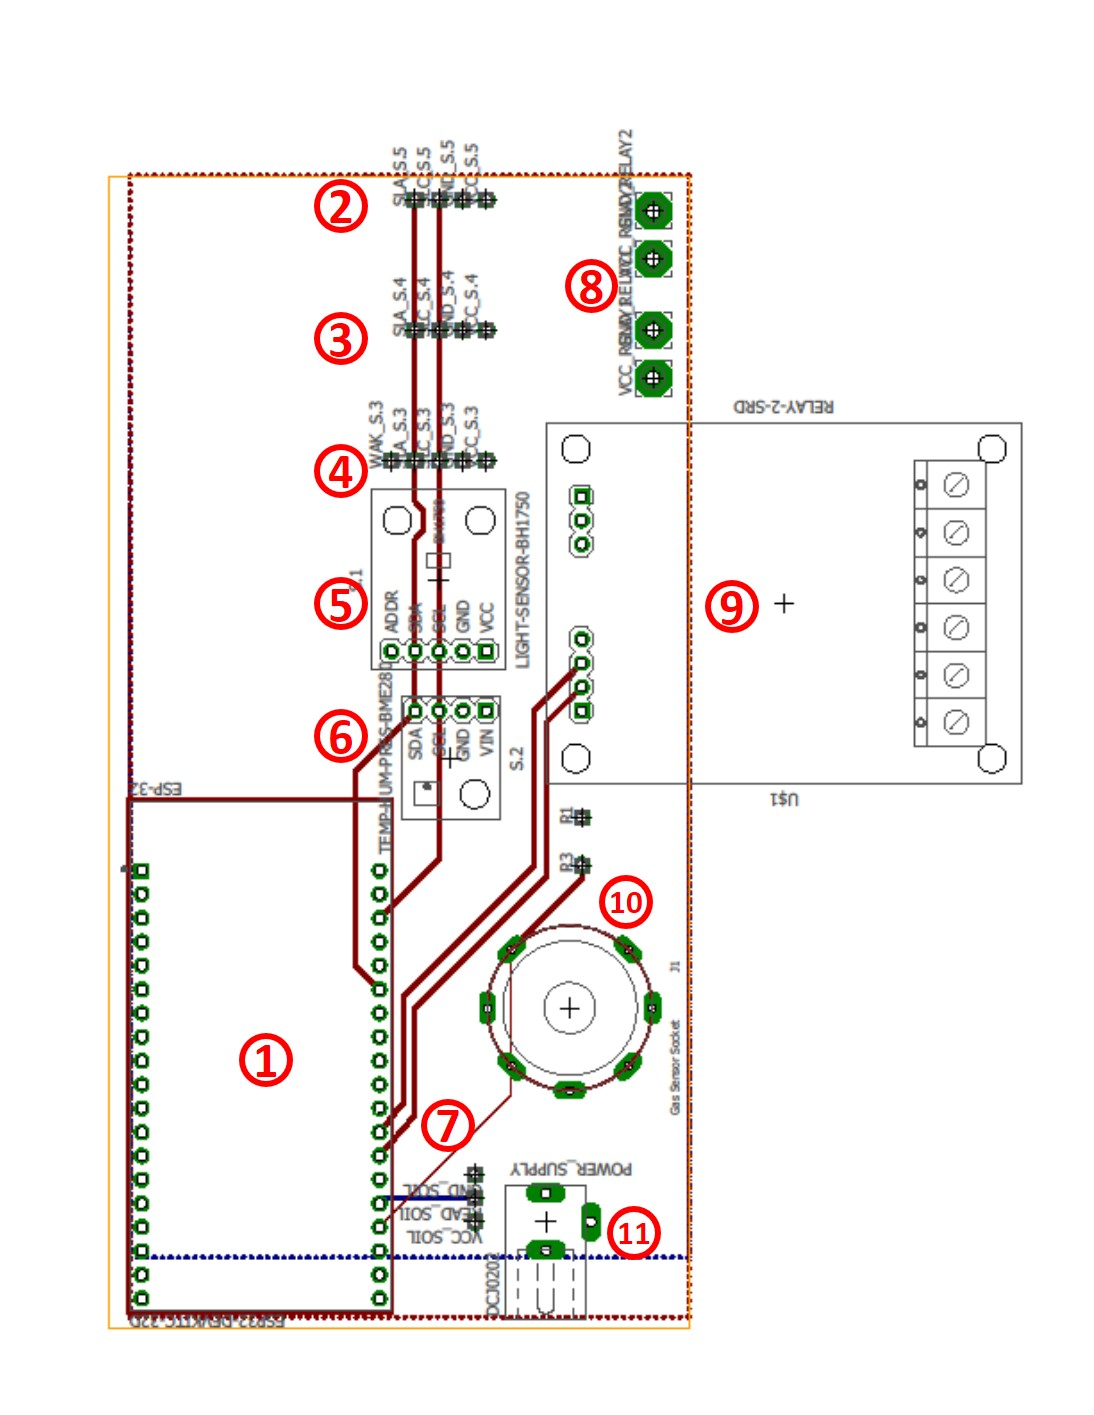
\includegraphics[width = 1\linewidth]{tomatoESPSchematic.jpg}
    \caption{Design of the climate sensor motherboard. The front and back of the motherboard have a +5V and GND plate respectively. The motherboard features the following components: (1) ESP-32 Development board, (2)-(6) I$^2$C connections for multiple sensor bake-out boards, (7) analog readout for a soil humidity sensor, (8) two power supplies for  auxiliary components. (9) Two relay circuit bakeout board to toggle auxiliary components, (10) analog readout for ozone sensor, (11) power supply socket.}
    \label{fig:ESP_motherboard}
\end{figure}
For the backbone of our home-made climate sensors we use an ESP-32 Development-board platform with integrated Bluetooth and Wi-Fi capabilities. It is cheaper compared to Arduino micro-controllers with similar features and is more suitable for permanent configurations as it has a smaller footprint. We designed a motherboard connecting the various climate sensors to the ESP-32 micro-controller itself avoiding electronic breadboards and jumper cables, which quickly become a mess. Figure\,\ref{fig:ESP_motherboard} shows the schematic of the climate sensor motherboard which facilitates up-to five I$^2$C connections to the ESP-32 micro-controller alongside analog connections to ozone and soil humidity sensors. The motherboard also provides sockets and connections for two relay switches, one of which is used to water the plants when the soil humidity readout is below a threshold value. The ESP-32 micro-controller runs a script that reads out each climate sensor available and presents the sensor values as characteristics in a Bluetooth Low Energy (BLE) server. A readout device (client) can connect to the BLE server and subsequently read-out the various climate parameters. In our case we use the previously mentioned Raspberry-Pi\,4 as a readout device, but for debugging purposes a phone using an appropriate application (e.g. nRF connect) can also be used to observe the climate parameters. The BLE server-client protocol is identical to how many wireless sports equipment works, such as, for example, heart rate chest band (BLE server) and a sports watch (BLE client). 
\subsection{Sensors}
The climate sensors are equiped with various individual sensors to monitor the climate within each growth container. Table \ref{Table: Sensors} gives an overview of the different sensors that we fit on the climate sensor motherboard to monitor the climate within each growth container.
\begin{table}[h]
\begin{tabular}{l|l|l|l}
\textbf{Measurement}                                                      & \textbf{Sensor}                                                         & \textbf{Range}                                                                                               & \textbf{Type} \\ \hline
\begin{tabular}[c]{@{}l@{}}Pressure\\ Temperature\\ Humidity\end{tabular} & BME280                                                                       & \begin{tabular}[c]{@{}l@{}}300-1100\,hPa\\ -40-85\,$^{o}$C\\ 0-100\%\,rel.\,hum\end{tabular}                                    & I2C                 \\ \hline
\begin{tabular}[c]{@{}l@{}}eCO2\\ VOC\end{tabular}                        & CCS811                                                                       & \begin{tabular}[c]{@{}l@{}}400-32768\,ppm\\ 0 - 29206\,ppb\end{tabular}                                                & I2C                 \\ \hline
Light                                                                     & BH175                                                                        & 0-65535  lx                                                                                                            & I2C                 \\ \hline
\begin{tabular}[c]{@{}l@{}}CO\\ NO$_2$\\ C$_2$H$_5$OH\\ VOC\end{tabular}    & \begin{tabular}[c]{@{}l@{}}Grove-Multichannel\\ Gas Sensor V2\end{tabular} & \begin{tabular}[c]{@{}l@{}}$\sim$5-5000\,ppm\\ $\sim$0-2\,ppm\\ $\sim$1-500\,ppm\\ $\sim$1-500\,ppm\end{tabular} & I2C                 \\ \hline
Ozone                                                                     & MQ131                                                                        & \begin{tabular}[c]{@{}l@{}}10-1000 ppb\\ The other one\end{tabular}                                                    & Analog              \\ \hline
Soil Humidity                                                             & Capacitive Sensor                                                            & 0-4096                                                                                                                 & Analog             
\end{tabular}
\label{Table: Sensors}
\caption{Overview  of the different sensors on the climate sensor motherboard. We give the measurement, type of the sensor, and the connection why which it is connected to the ESP-32 micro-controller.}
\end{table}

\section{Data Collection}
\subsection{Methods of Acquisition}
The plant growth facility supports various methods of data collection through different channels and at different rates of acquisition. The following methods can be used for climate data collection and logging:
\begin{enumerate}
    \item The Linux job-scheduler Cron periodically runs a homemade python script on the Raspberry-Pi\,4 that reads out all the relevant sensors on each ESP-32 sensor board. The python script subsequently uploads the sensor readouts into the database where the data is stored. The maximum rate at which the Cron job scheduler is able to run the readout script is once per minute.
    \item Manually running a streaming script on the Raspberry-Pi\,4 to continually read out the relevant sensors on the climate sensor board. Identical to the first method the streaming script subsequently uploads the received sensor values into the database for storage and remote visualisation. The streaming script can be configured to (I) readout a single climate sensor or (II) readout all available climate sensors. This data acquisition mode results in a measurement every 2 seconds, or a measurement rate of 0.5\,Hz.
    \item The final method of data acquisition is to connect a single sensor board to a computer and establish a serial connection. The ESP-32 boards are programmed to print the sensor values at the refresh-rate of the micro-controller firmware ($\sim2$\,Hz). This method was originally intended for debugging the firmware of the ESP-32, however it can also be highly advantageous to see fast, dynamic changes within the growing facility. The downside of this acquisition mode it that the sensor measurements are not stored automatically in the database. Data taken through this acquisition mode needs an external program if it needs to be saved for later use. 
\end{enumerate}
The Cron based data acquisition method is ideal for continuous observation of the overall climate within the plant growth facility and runs continually. The two other acquisition methods are ideal for fast observation of dynamic processes in circumstances when external measurement devices are sampling within the growth chamber and these data steams have to be initiated manually.

\subsection{Database and data visualization}
We use InfluxDB as the database structure to store and handle the data from the plant growing facility. InfluxDB is an open-source database structure optimised for handling time series data. It allows high throughput data logging and native data analysis. The structure requires data to be written as JSON objects which can be added to the database. The JSON objects contain the measurement time, location within the plant-growing facility, and the respective measurement values. The database can be queried to selectively return data for subsequent analysis. To continually visualize the data stream from the growing compartments  the ESP-32 sensors we use a Grafana dashboard. Grafana is an open source analytic and interactive visualization web application. It provides charts, graphs, and alerts for the growth chamber. The Grafana service is hosted on the Raspberry-Pi\,4 and accessible for viewing to everyone on the institutes network accessible via IP address and port 10.106.9.83:3000.
\section{Characterisation measurements}
\begin{figure*}
    \centering
    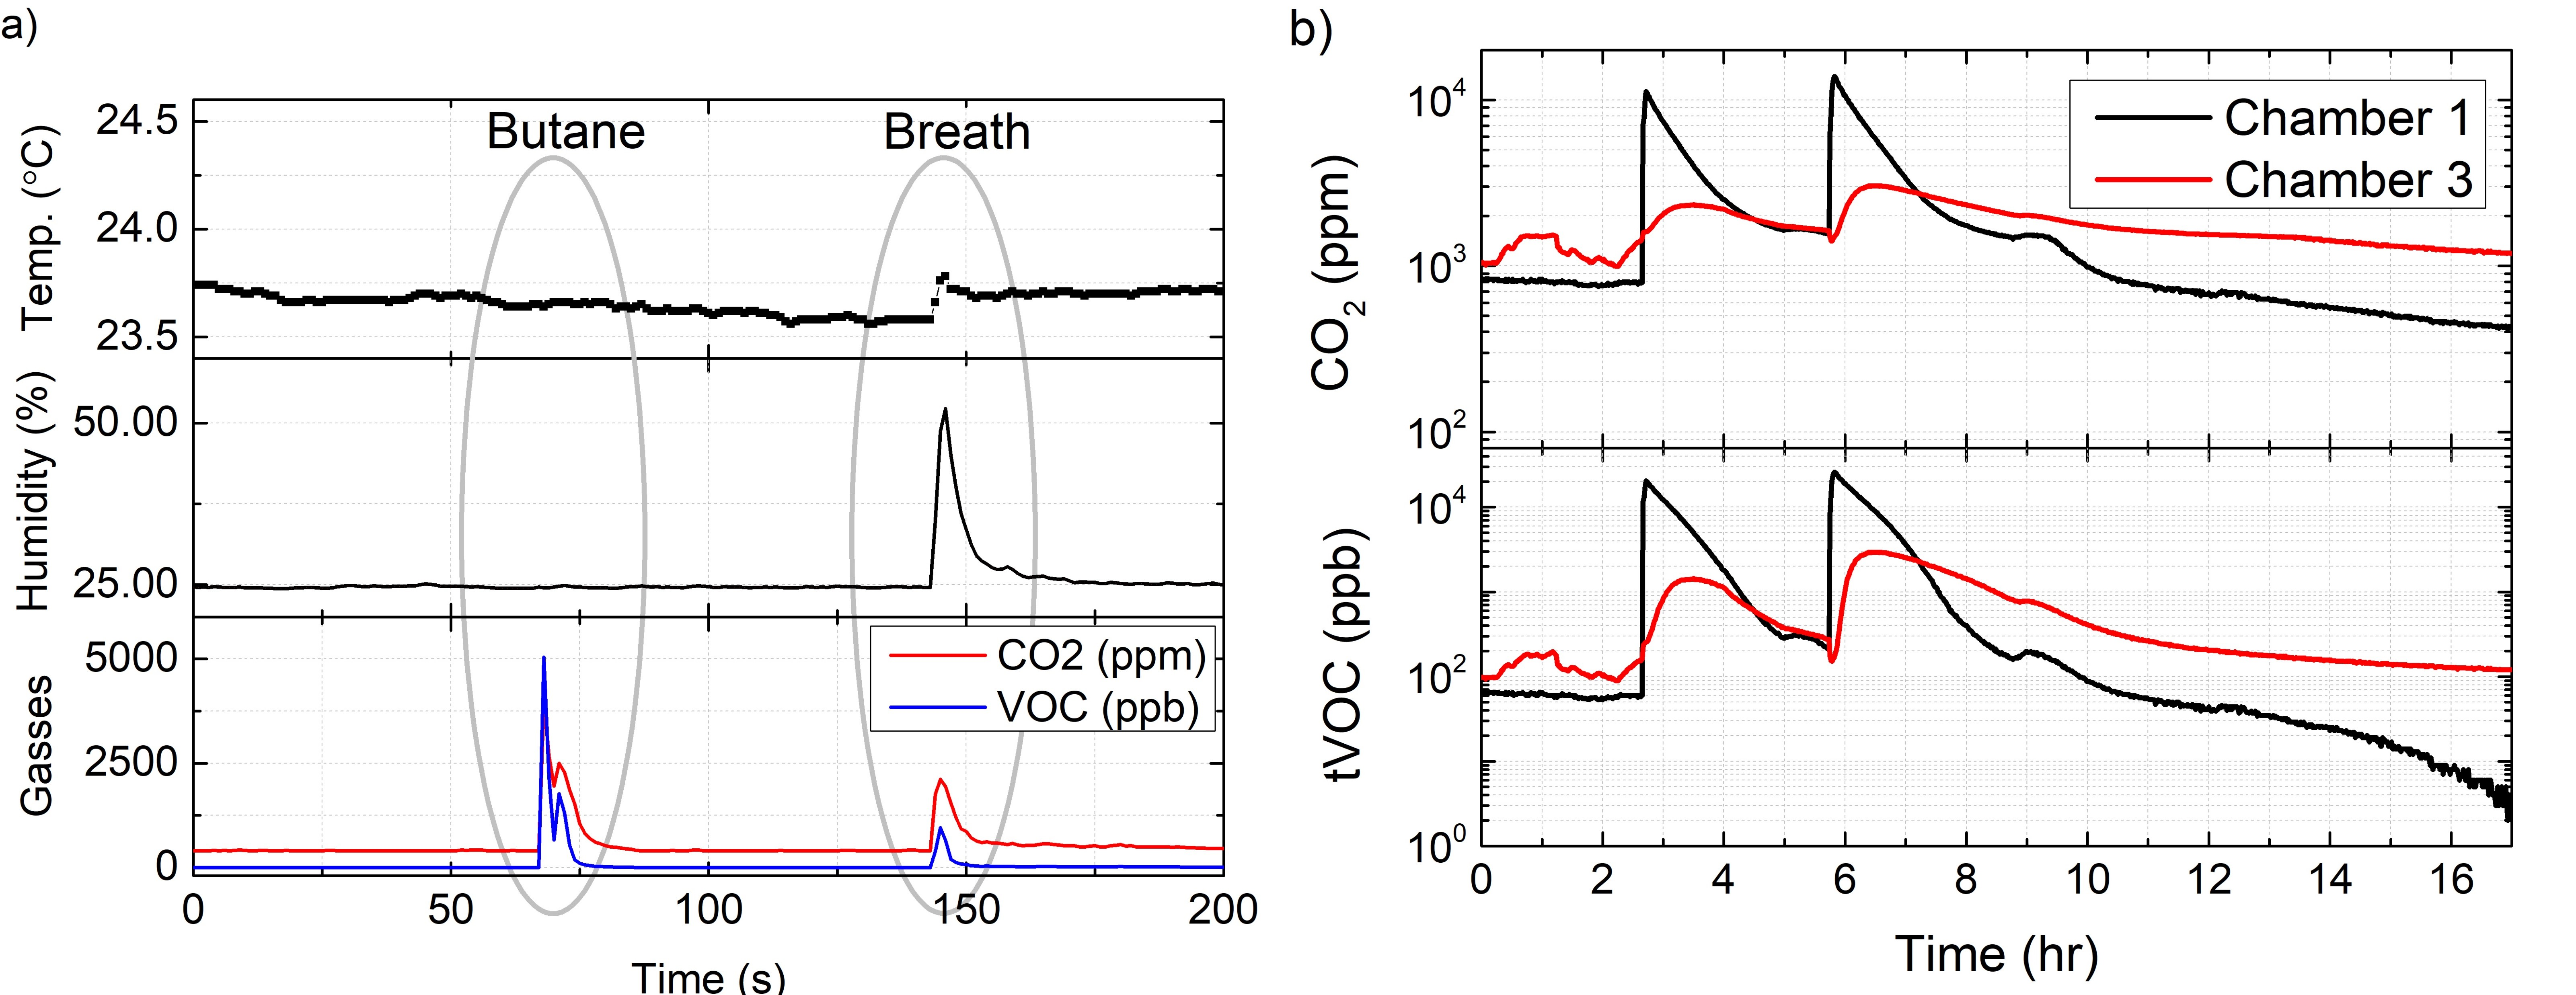
\includegraphics[width = \textwidth]{test_measurements.jpg}
    \caption{Characterization measurements of the ESP32 sensor-board and plant growing facility as a whole. \textbf{(a)}.  Consecutive exposures of climate sensor to butane and respiration. The butane is only registered with an increase of the measured CO$_2$ and tVOC concentrations by the CSS811 sensor, whereas the exhaled breath is also measured to have a higher temperature (top) and relative humidity (bottom). \textbf{(b)}. Measured CO$_{2}$ (top) and tVOC (bottom) concentrations in growth chambers 1 and 3 over a period of 17 hours. At t$\,=\,2.7$\,Hr and t$\,=\,5.75$\,Hr a petri-dish with a $\sim$ml of methanol is introduced into growth chamber 1. The CO$_{2}$ and tVOC concentrations are monitored as the methanol evaporates and diffuses through the entire growing facility. The measured CO$_{2}$ and tVOC concentrations in chamber 1 spike up immediately and slowly, over the course of a couple of hours, decay to their ambient levels. In chamber 3, the CO$_{2}$ and tVOC concentrations rise, albeit more slowly and not as drastically as in chamber 1. The highest level of recorded concentrations measured in chamber 3 are an order of magnitude lower than the maximum concentrations measured in chamber 1. Moreover, the time delay between the highest measured CO$_2$ and tVOC concentrations is approximately 45 minutes.}
    \label{fig: baseline Butane and leaktesting}
\end{figure*}
Characterization measurements are crucial for the operation of the plant-growing facility and for the understanding of future plant emission studies. To explain deviations from baseline conditions, those baseline conditions should be known and well understood. In Fig.\,\ref{fig: baseline Butane and leaktesting} we show two distinct characterization measurements. Figure\,\ref{fig: baseline Butane and leaktesting}(a) shows response of the climate sensor to exposure to two  distinctly different conditions, human respiration and gaseous butane. We are able to distinguish between these two exposures by identifying temperature and humidity changes in the case of exposure to human respiration and the subsequent absence absence of those changes in the exposure to gaseous butane whereas both respiration and butane register on the tVOC sensor. Figure\,\ref{fig: baseline Butane and leaktesting}(b) shows the measured CO$_2$ and tVOC concentrations in growth chambers 1 and 3 over a period of 17 hours as an amount of methanol is introduced twice (at t = $2.7$\,hr and t = $5.75$\,hr) into chamber 1 and subsequently evaporates. The evaporation is registered on by the CO$_2$ and tVOC sensor on the climate sensors. The better the insulation between chambers 1 and 3, the slower the rise of CO$_2$ and tVOC concentrations will be in chamber 3. We observe that their concentrations do rise, albeit more slowly as in chamber 1. Furthermore, the the highest level of  concentrations measured in chamber 3 are an order of magnitude lower than the maximum concentrations measured in chamber 1. Most importantly, the time delay between the highest measured CO$_2$ and tVOC concentrations is approximately 45\,minutes. This means that any plant-to-plant signalling though VOC emissions will have a significant time delay and will not disturb control measurements taken at the same time as plant affliction measurements.  
The final characerization measurement, shown in Fig.\,\ref{fig:long observation}, shows 10 day-night cycles of chambers 1 and 3 in the plant-growing facility. The parameters given include temperature, relative humidity, light level, CO$_2$ concentrations and tCOV concentrations. For all parameters except the latter two, the baseline/ambient lab levels are also recorded. Presence of people in the lab can be tracked by the lab lights sporadically switching on/off. From the 10-day observation a clear relation between the temperature in the growth compartments and the on/off status of the light can be seen, the growing lights are also responsible for lowering the relative humidity during day cycles. A high degree of temperature isolation is achieved through the reflective aluminium foil which lines the inside of each growth compartment and no temperature increase in growth chamber 1 can be observed while extra growing lights in box 3 are turned on to simulate``\textit{high noon}" conditions. 
\begin{figure*}
    \centering
    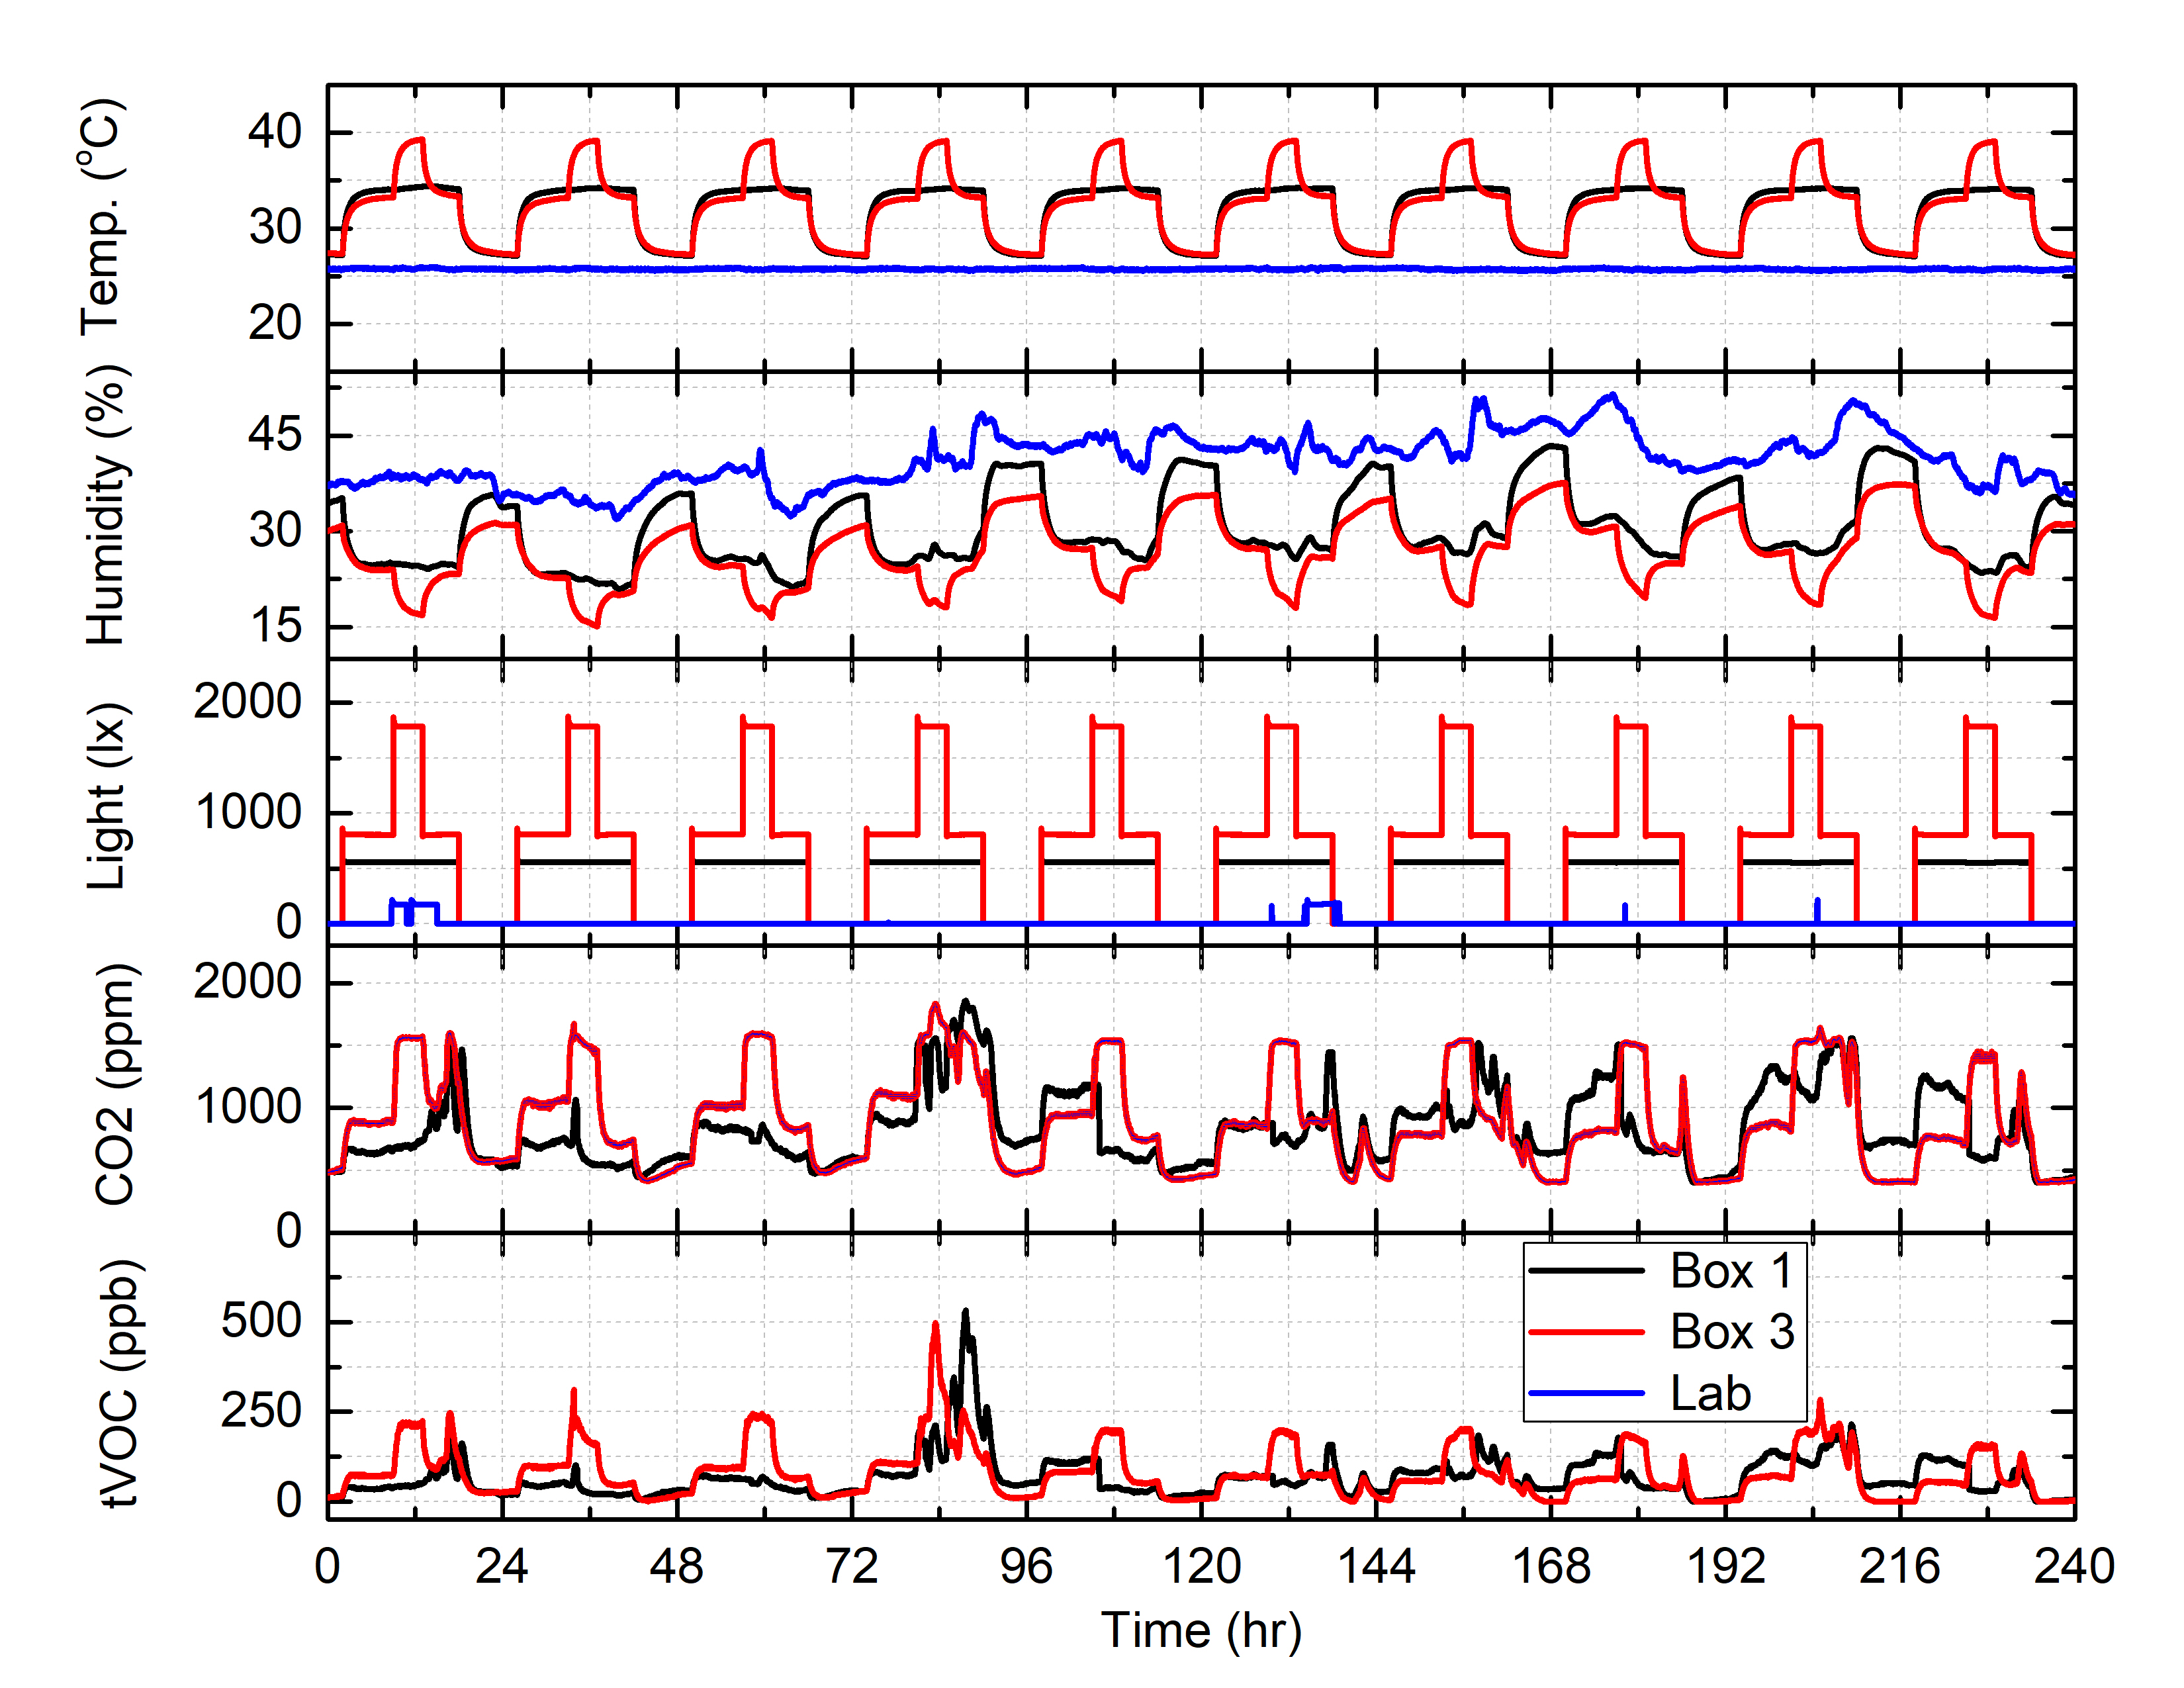
\includegraphics[width = 1.2\textwidth, angle = -90]{10d measurement.jpg}
    \caption{Observation of the climate parameters in growth boxes 1 (Black line), 3 (Red line) and the ambient lab environment (Blue line) over a continuous period of 10 days (240 hours), starting t\,$=0$ at 30-07-2021 00:00 until 09-08-2021 00:00. A clear correlation between the temperature and humidity within each box and the on/off status of the growing lights can be identified. Measured CO$_2$ and tVOC concentrations in the growth cambers are also highly correlated to the applied light cycle. Additional growing lights are turned on in box 3 for 4 hours each cycle to simulate high noon.}
    \label{fig:long observation}
\end{figure*}
\newpage

\section{Outlook \& Conclusion}
In summary, this work shows a design, realisation and characterization of a cost-effective plant-growth facility with integrated monitoring capabilities. We show the data acquisition, handling and visualisation scheme of the facility and demonstrate a couple of characterizing measurements that are important for its application. Importantly, all the software associated to the growth-facility, such as the ESP-32 firmware and the data acquisition scripts are freely available on the GitHub development platform (\url{https://github.com/JCVis/weatherstation}) and will be updated as improvements are made to the growth facility and as inspiration for other designs. Future work will include more characterizations of the growing facility containing plants, the subsequent growing of plants from seeds and various plant VOC emission studies are planned with this plant-growing facility.
\section*{Acknowledgements}
We would like to thoroughly thank the Max Planck Institute for Chemistry in Mainz, and specifically Prof. Jonathan Williams, Joseph Byron and the mechanical workshop of the MPIC for funding and fabricating the plant-growing facility.
\end{document}